% =====================================================================
% Figure captions for synopsis-genomic-scripting.tex
%
% Every number quoted below is produced by figures/generate_panels.py,
% which recomputes each quantity from validation/core.py,
% validation/semantics.py and validation/lang.py at plot time rather
% than reading validation/results/*.json. The panels are therefore an
% independent second execution of the framework, not a redraw of the
% validation suite's output; where a panel agrees with the suite, that
% agreement is evidence. Seed 20260816 throughout; minimum cuts are
% computed exactly by enumeration over separating subsets, never
% approximated by a max-flow routine.
%
% \input this file, or paste the blocks into the body where wanted.
% =====================================================================

\begin{figure*}[!htbp]
    \centering
    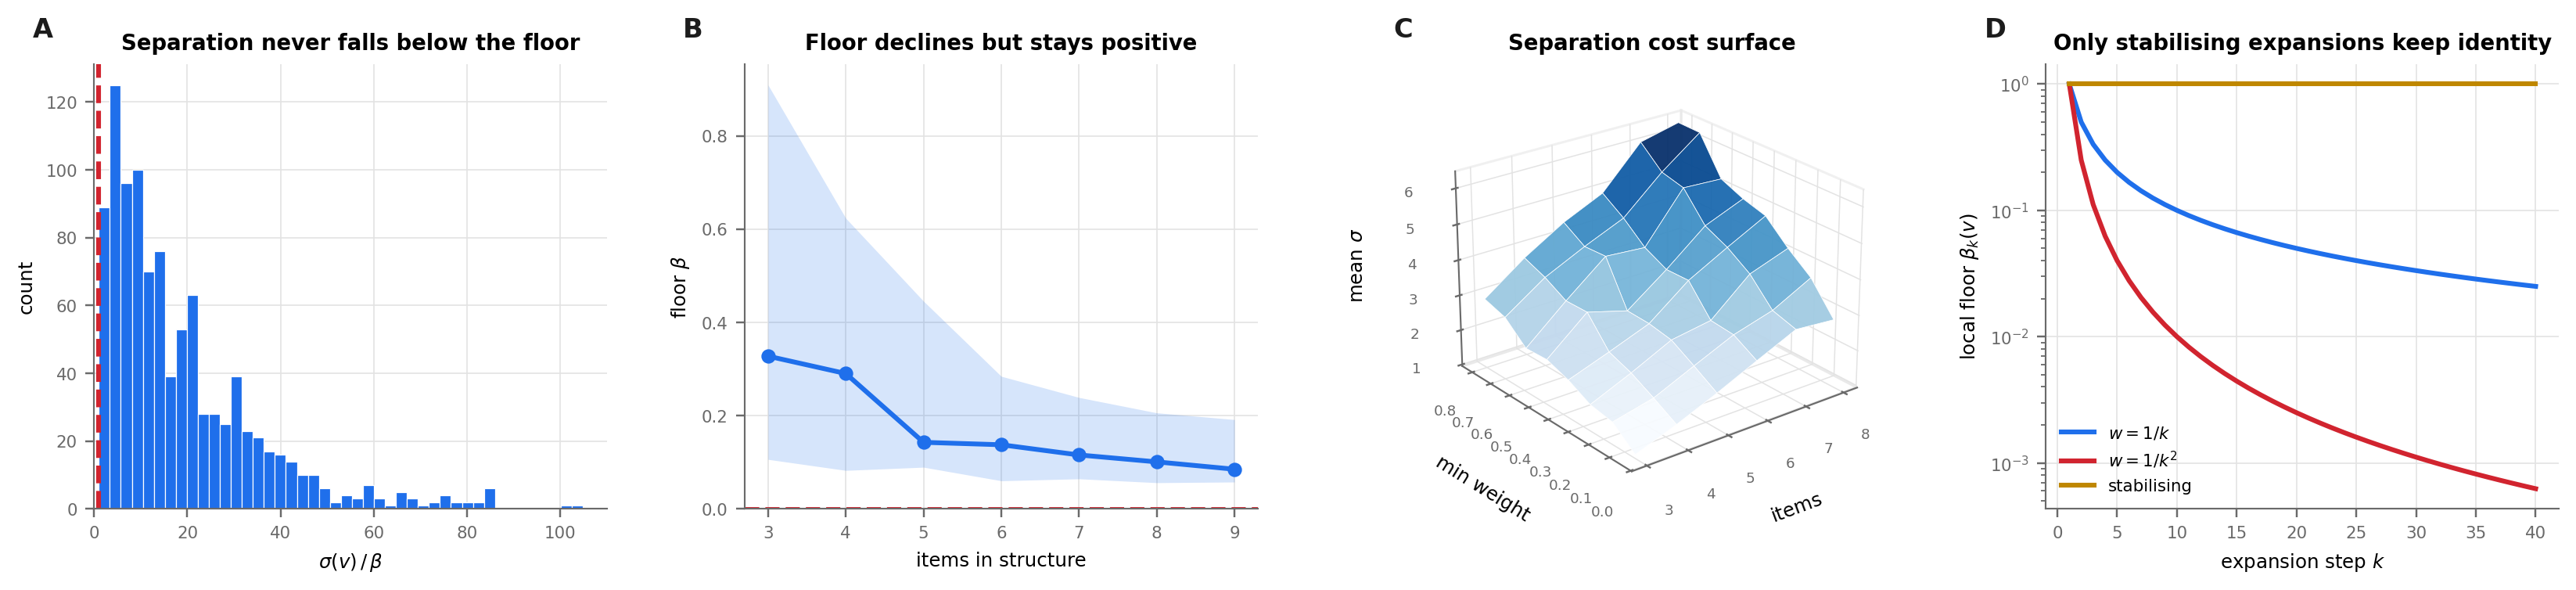
\includegraphics[width=\textwidth]{figures/panel_1_floor.png}
    \caption{\textbf{The floor: every distinction has a strictly positive price, and that price survives expansion only conditionally.}
    All quantities are computed on finite weighted graphs with strictly positive edge weights (\Cref{def:fwg}); minimum cuts are exact, obtained by enumeration over all separating vertex subsets rather than by an approximate max-flow routine, so no agreement below can be a solver artefact.
    (\textbf{A})~Distribution of $\sep(v)/\flo$ over $997$ items drawn from random contact structures of $3$--$6$ items. The ratio never falls below $1$ in any instance (minimum exactly $1.000$, median $13.38$, maximum $104.9$), which is \Cref{thm:floor}: the separation cost of an item is at least the contact floor. The mass at the left edge is the set of items whose cheapest cut is the floor edge itself; the long right tail is items embedded in dense neighbourhoods, whose boundary is correspondingly expensive. That the minimum is exactly $1$ and not $0.999$ is the point --- the bound is attained, not merely approached.
    (\textbf{B})~The floor $\flo$ against structure size, median with the $10$--$90$ percentile band. The median falls monotonically from $0.328$ to $0.085$, because each additional item contributes further edges and the floor is a minimum over a growing set. It does not reach zero, and cannot: the minimum of a finite set of strictly positive weights is positive. The declining trend and the strict positivity are both essential and are easily conflated, which is why the band rather than the median alone is drawn --- a floor that shrinks is not a floor that vanishes.
    (\textbf{C})~Mean separation cost as a surface over the number of items and the minimum admissible edge weight, each cell a mean over independent structures. The surface ranges over $1.06$--$6.36$ and is bounded away from zero throughout, exhibiting \Cref{thm:floor} as a property of the parameter space rather than of particular instances.
    (\textbf{D})~The local floor $\flo_k(v)$ of \Cref{def:localfloor} under three expansion regimes (\Cref{def:expansion}), logarithmic axis. Adding edges at $v$ of weight $1/k$ drives the local floor to $2.5\times10^{-2}$ by step $40$ and $1/k^2$ drives it to $6.3\times10^{-4}$, while a stabilising expansion holds it at $1.0$. This is the content of \Cref{rem:not-positive}: the \emph{unconditional} claim that the floor is preserved under expansion is false --- an item can dissolve into the medium in the limit --- and \Cref{thm:floorpres,thm:invariance} are therefore stated under the floor-stabilising hypothesis of \Cref{def:stabilising}. The two decaying curves are the counterexample the theorem must exclude, plotted rather than described.}
    \label{fig:panel1}
\end{figure*}

\begin{figure*}[!htbp]
    \centering
    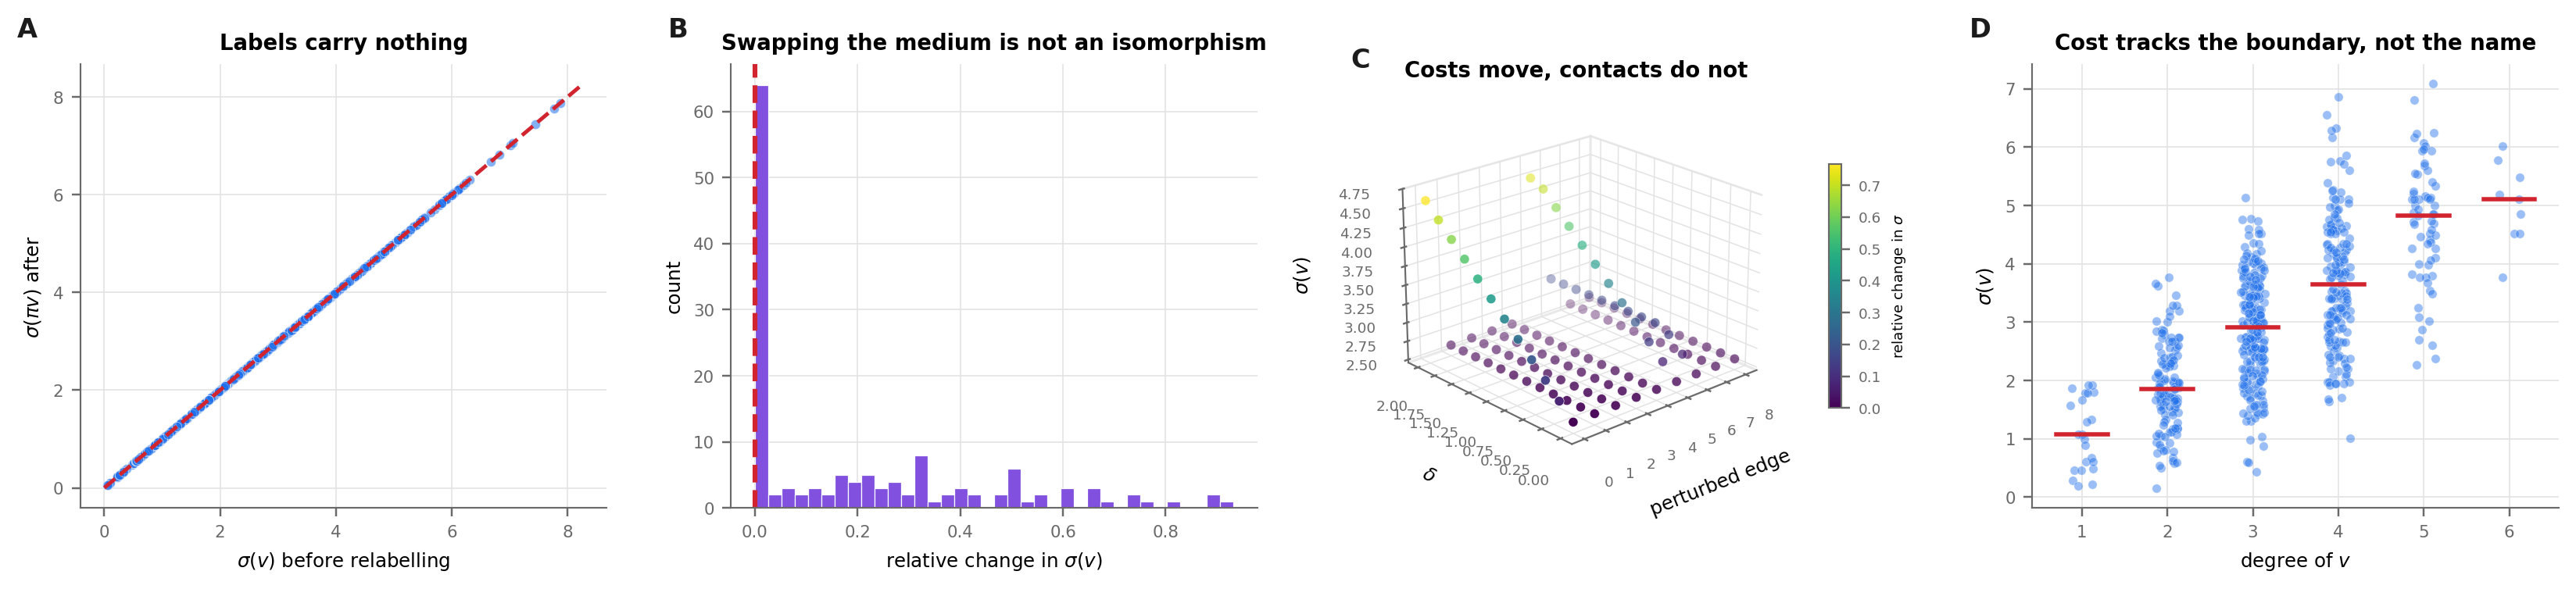
\includegraphics[width=\textwidth]{figures/panel_2_invariance.png}
    \caption{\textbf{The invariant is borne by the cut, not by the label: names are free, the medium is not, and perturbation moves costs without touching contacts.}
    (\textbf{A})~Separation cost before against after a random relabelling, for $748$ items. Every point lies on the identity diagonal: the maximum absolute deviation is exactly $0$, not merely small. A weighted isomorphism carries cuts to cuts weight-for-weight, so $\sep$ is preserved (\Cref{thm:invariant-cut}) while the vertex labels have been permuted --- the invariant and the name come apart, which is \Cref{cor:labels}. This is the formal reason a sequence, being a labelling, cannot carry what a comparison of sequences is asked to recover.
    (\textbf{B})~The same experiment with one clause of \Cref{def:iso} withdrawn. Swapping the medium's role with an ordinary item is not a weighted isomorphism, and the invariance duly fails: over $140$ structures the relative change in $\sep(v)$ is non-zero in $55.0\%$ of cases, mean $0.198$, with the dashed line marking the zero that (\textbf{A}) achieves everywhere. The requirement that an isomorphism fix the medium is not a technical convenience; it is what makes \Cref{thm:invariant-cut} true, and this is what its removal costs.
    (\textbf{C})~Separation cost under per-edge perturbation (\Cref{def:perturbation}), $9$ edges swept against perturbation magnitude $\delta$, coloured by relative change in $\sep(v)$. Costs move --- up to $0.768$ relative --- while the edge set is fixed throughout the sweep: the skeleton is invariant, verified programmatically at every point rather than asserted (\Cref{prop:skeleton}). Perturbation makes distinctions dearer and never creates or destroys a contact, which is exactly the sense in which a variant has an effect without rewriting what is adjacent to what.
    (\textbf{D})~Separation cost against the degree of $v$ over $597$ items, with per-degree medians. Cost tracks the size and weight of an item's boundary, not any property of its name; the spread within each degree is the contribution of the weights, and the trend across degrees is the contribution of the boundary. Read with (\textbf{A}), this is \Cref{rem:bearing}: what individuates an item is where it sits, and every quantity in the framework is downstream of that.}
    \label{fig:panel2}
\end{figure*}

\begin{figure*}[!htbp]
    \centering
    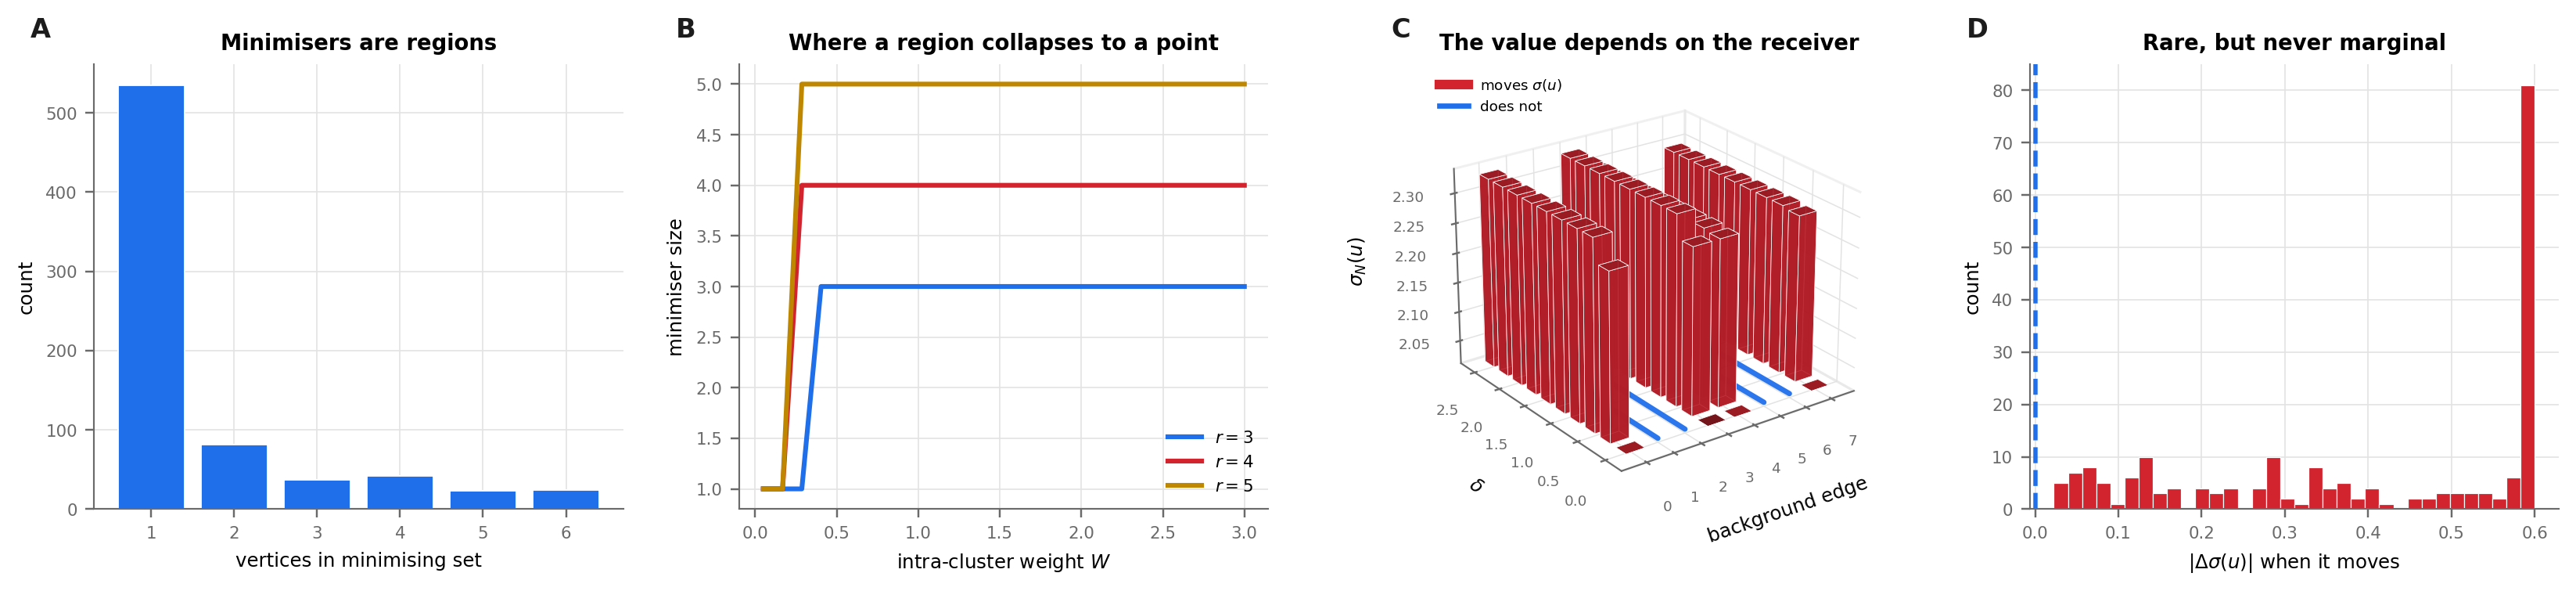
\includegraphics[width=\textwidth]{figures/panel_3_region_receiver.png}
    \caption{\textbf{Identity is regional rather than pointwise, and the value an item registers depends on the receiver that registers it.}
    (\textbf{A})~Sizes of the minimising $(v,\med)$-separating set over random contact structures. The mode is the singleton and $72.1\%$ of minimisers are of that form, but $27.9\%$ detach a neighbourhood rather than the item alone. That minority is what \Cref{thm:region} asserts and what \Cref{cor:notpoint} needs: identity is not \emph{in general} attributable to a point. The claim is not that a pointwise reading usually fails --- it usually succeeds --- but that it fails often enough, and without warning, that a framework may not assume it. The distribution is drawn in full rather than summarised by its mode for exactly this reason.
    (\textbf{B})~Where a region collapses to a point. Minimiser size against intra-cluster weight $W$ for $r\in\{3,4,5\}$, in the two-cluster family. At low $W$ the cheapest cut takes the whole cluster; as $W$ rises, severing intra-cluster edges becomes expensive relative to the item's own medium edge and the minimiser drops to a singleton. The crossover is not a pathology but the boundary between the two regimes, and it is what \Cref{rem:badwitness} records mistaking: assuming a light edge between two items places them at the floor invalidated our first witness for \Cref{thm:falsefriend}.
    (\textbf{C})~Receiver-relativity made concrete (\Cref{def:receiver}). The separation cost $\sep_N(u)$ of a fixed item is plotted over $8$ \emph{background} edges --- none incident to $u$ --- each swept over a perturbation magnitude $\delta$. Four of the eight move $\sep_N(u)$; the other four leave it exactly constant and are drawn as flat marker lines at the unperturbed value, so that absence of response is visible as a response rather than collapsing into the baseline. The value of an item is therefore a property of the item \emph{and} its receiver, not of the item alone, which is \Cref{thm:receiver}.
    (\textbf{D})~The magnitude of that dependence when it occurs. Sweeping a perturbation across every non-incident edge of a population of random contact structures, $206$ of $1181$ edges ($17.4\%$) moved $\sep(u)$ at all; where an edge did move it, the smallest displacement recorded was $0.022$. Disagreement between receivers is thus a minority event by construction --- a background edge moves the cost only when it crosses the minimising cut --- but it is never marginal when it happens. The displacements are broadly spread rather than concentrated, yet bounded away from zero: either receivers agree exactly, or they disagree by an amount no measurement programme will close. There is no population of near-misses in between, which is precisely what a noise account would predict and is why \Cref{cor:notnoise} is substantive (\Cref{rem:receiverrate}; \Cref{sec:validation}, E10, independently reports $26$ of $150$ receiver pairs disagreeing, $17.3\%$, smallest substantial difference $0.056$).}
    \label{fig:panel3}
\end{figure*}

\begin{figure*}[!htbp]
    \centering
    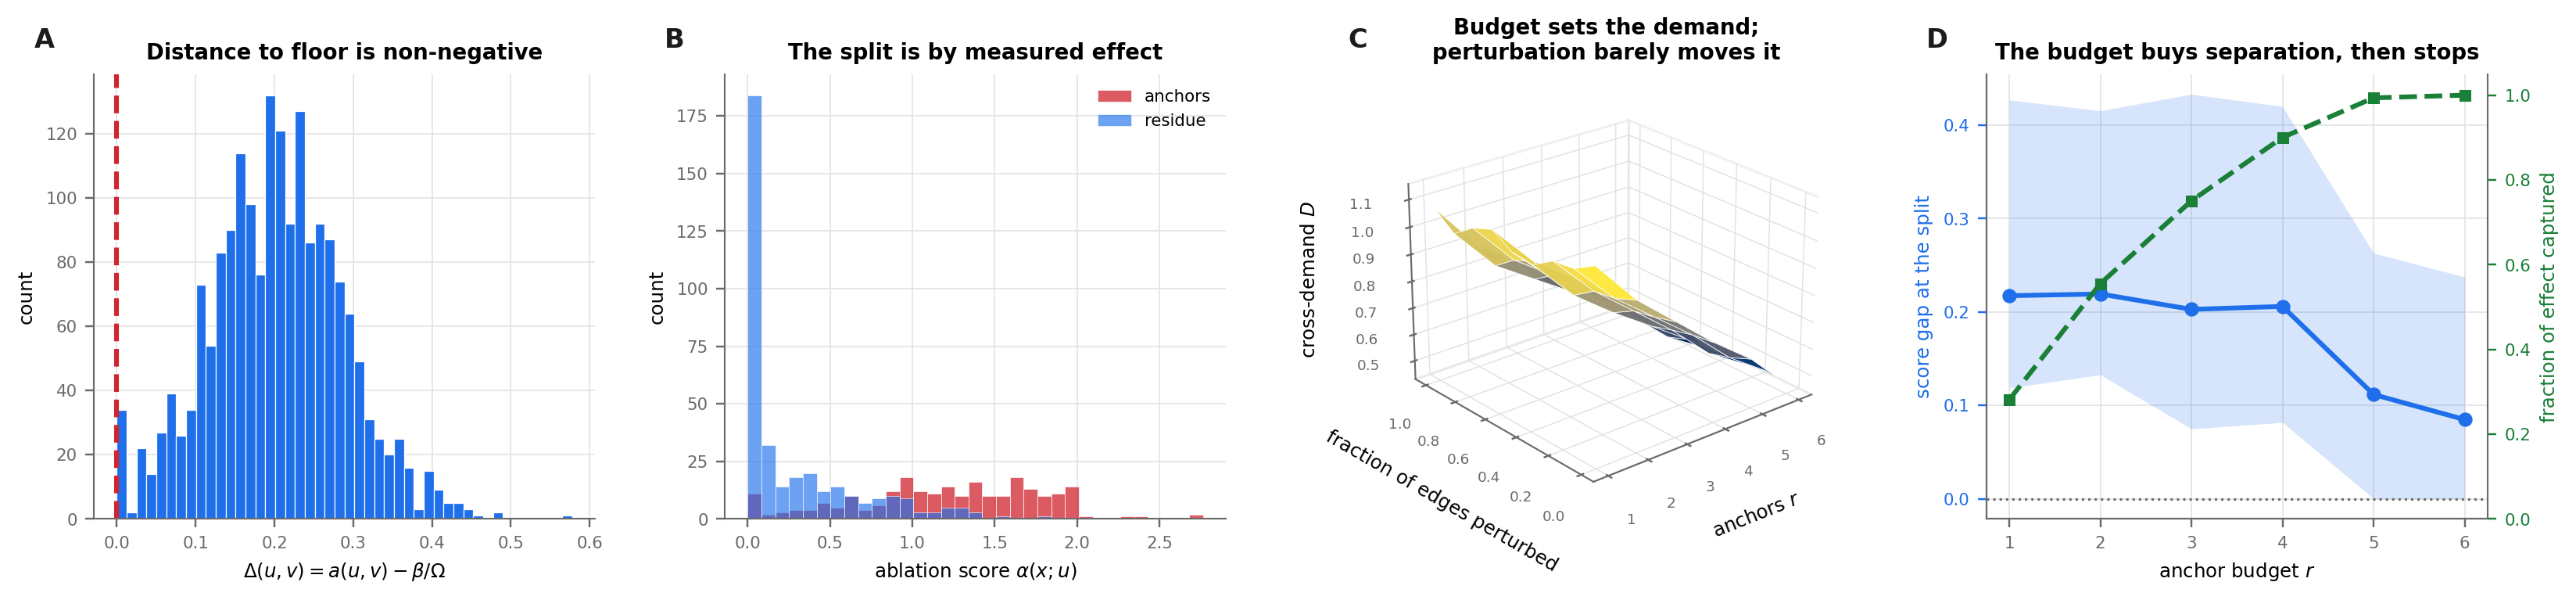
\includegraphics[width=\textwidth]{figures/panel_4_alignment.png}
    \caption{\textbf{Alignment is measured as distance to the floor, the anchor/residue split is made by measured effect, and the anchor budget is what sets the demand.}
    (\textbf{A})~Distribution of the distance to the floor $\Delta(u,v)=a(u,v)-\flo/\Om$ over $1871$ pairs (\Cref{def:alignment}). The minimum is exactly $0$ and no value is negative, which is \Cref{prop:nonneg}. The $1.6\%$ of pairs sitting exactly at zero are separated precisely at the floor --- the cheapest distinction the structure admits. That such pairs exist and are not rare is what makes \emph{sufficient} alignment a meaningful target: two units may sit at the floor and still cost $\flo>0$ to tell apart, so quiescence at $\theta=0$ never means indistinguishability.
    (\textbf{B})~The anchor/residue split of \Cref{def:anchor}, as overlaid distributions of the ablation score $\alpha(x;u)=\sep_\Gph(x)-\sep_{\Gph\setminus u}(x)$. Anchors have median score $1.231$ against the residue's $0.069$ --- a separation of more than an order of magnitude in the median. The split is therefore by measured effect on separation cost, not by annotation, name or position, and the deterministic tie-break on names makes it reproducible without making it label-dependent (\Cref{cor:resacc}).
    (\textbf{C})~Cross-demand $\dem$ (\Cref{def:crossdemand}, \eqref{eq:demand}) as a surface over the anchor budget $r$ and the fraction of edges perturbed, on $11$-item structures. Demand ranges over $0.444$--$1.142$, but the two arguments are not comparable in their effect: the mean span over the budget axis is $0.609$ against $0.092$ over the perturbation axis, a ratio near seven to one. The budget sets the demand and perturbation barely moves it. We report the asymmetry rather than engineer it away --- the shallowness in one direction is a finding about what cross-demand is sensitive to, and the title of the axis states it.
    (\textbf{D})~What the anchor budget buys, and where it stops. The gap between the lowest anchor score and the highest residue score (median with interquartile band, left axis) falls from $0.218$ at $r=1$ to $0.085$ at $r=6$, while the fraction of total ablation effect captured by the anchors (right axis) rises from $0.282$ to $1.000$. Enlarging the budget therefore captures more of the effect but buys progressively less separation at the split; the two axes together say that $r$ is a genuine parameter with a diminishing return, not a threshold to be tuned until a verdict changes. Structures are drawn at $11$ items so the budget stays strictly inside the available set: where the residue empties, the gap is undefined rather than zero, and the code raises instead of plotting a fabricated point.}
    \label{fig:panel4}
\end{figure*}

\begin{figure*}[!htbp]
    \centering
    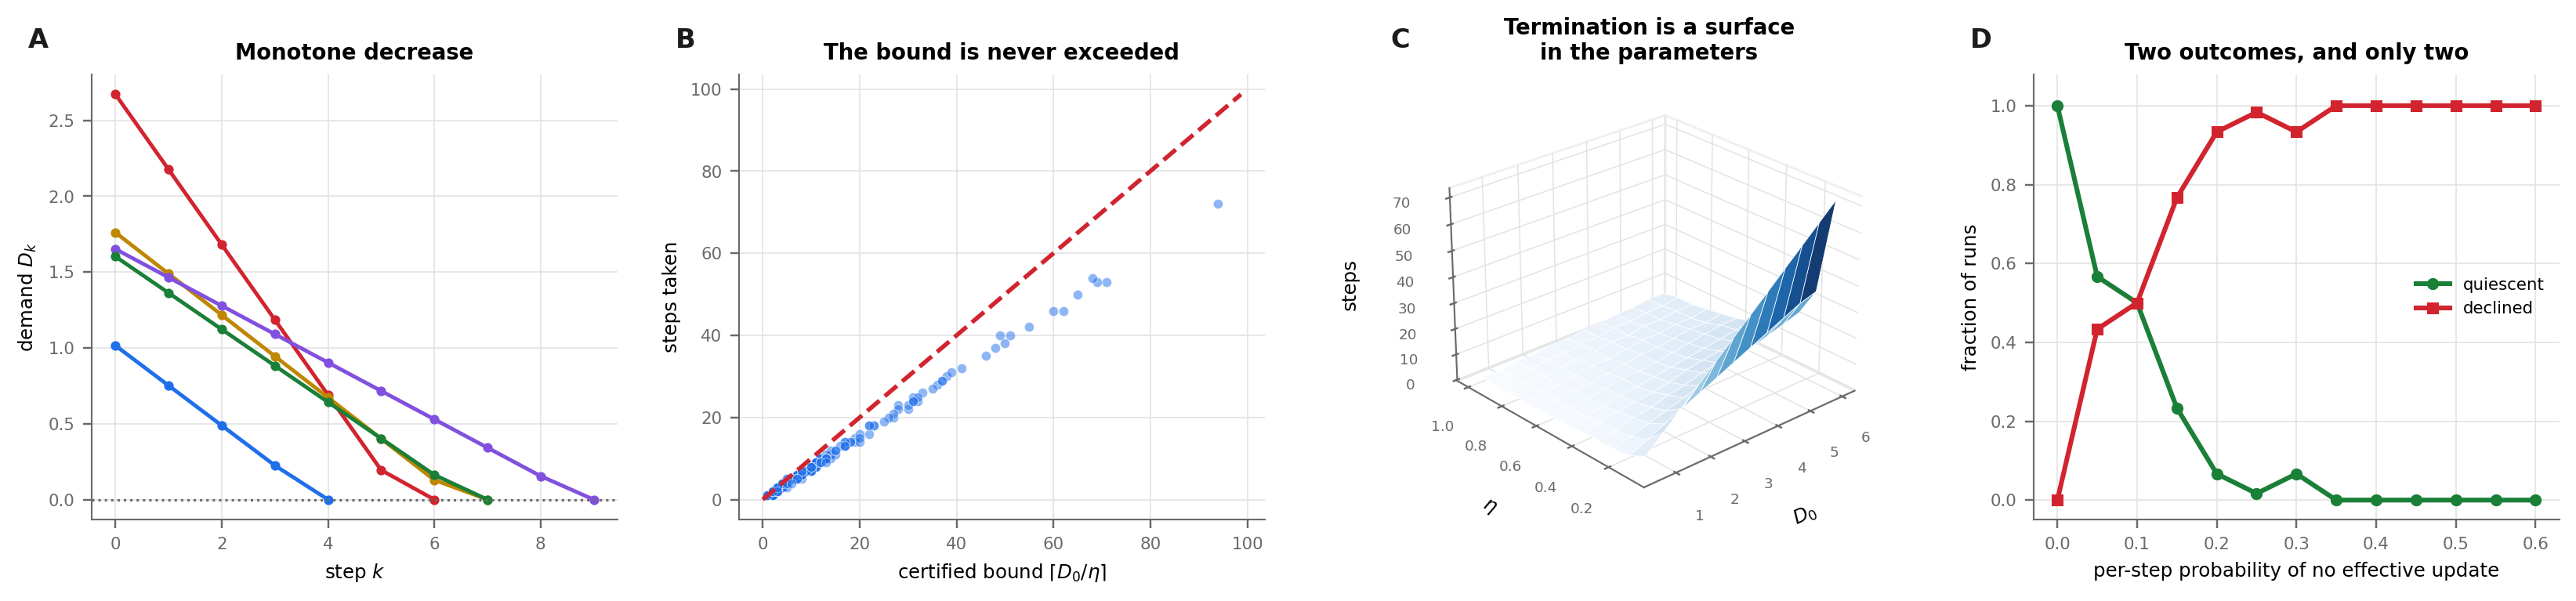
\includegraphics[width=\textwidth]{figures/panel_5_relaxation.png}
    \caption{\textbf{Relaxation decreases monotonically, terminates within a bound computable before the loop is entered, and does so in exactly two ways.}
    (\textbf{A})~Demand trajectories $\dem_0>\dem_1>\cdots$ under the effective-update assumption (\Cref{ass:effective}). Every trajectory is strictly decreasing while defined, which is \Cref{thm:mono}. No trajectory rises, stalls, or oscillates: the update either buys at least $\eta$ of progress or lands at or below the threshold $\theta$, and the disjunctive form of the assumption is what admits the final step without demanding a full $\eta$ from it (\Cref{rem:lastdisjunct}).
    (\textbf{B})~Realised step count against the certified bound $\lceil \dem_0/\eta\rceil$ emitted by the compiler, with the line $y=x$. Over $260$ runs there are $0$ violations --- no point lies above the diagonal. The bound is not a heuristic estimate but a consequence of \Cref{thm:mono}, and it is computable from values in scope at the point the loop is written, which is what lets a synopsis program state its own cost before running (\Cref{thm:total}).
    (\textbf{C})~Steps to termination as a surface over the initial demand $\dem_0$ and the guaranteed decrement $\eta$. Termination is a property of the parameter pair rather than of the instance: the surface rises in $\dem_0$ and falls in $\eta$, tracking $\lceil \dem_0/\eta\rceil$ across the plane. There is no region of the parameter space in which the loop fails to terminate, which is the practical content of \Cref{thm:dichotomy}.
    (\textbf{D})~The dichotomy itself. As the per-step probability of no effective update rises from $0$ to $0.6$, runs move from quiescence to decline; at every sampled probability the two fractions sum to exactly $1$, verified numerically rather than by inspection. There is no third outcome --- no divergence, no silent non-termination, no run that neither reaches $\theta$ nor reports that no effective update exists. Decline is a reported verdict and not a failure (\Cref{rem:decline}): the experiment runs to completion and says what happened, which is what \textsf{DECLINE} is for in the four-column criterion.}
    \label{fig:panel5}
\end{figure*}

\begin{figure*}[!htbp]
    \centering
    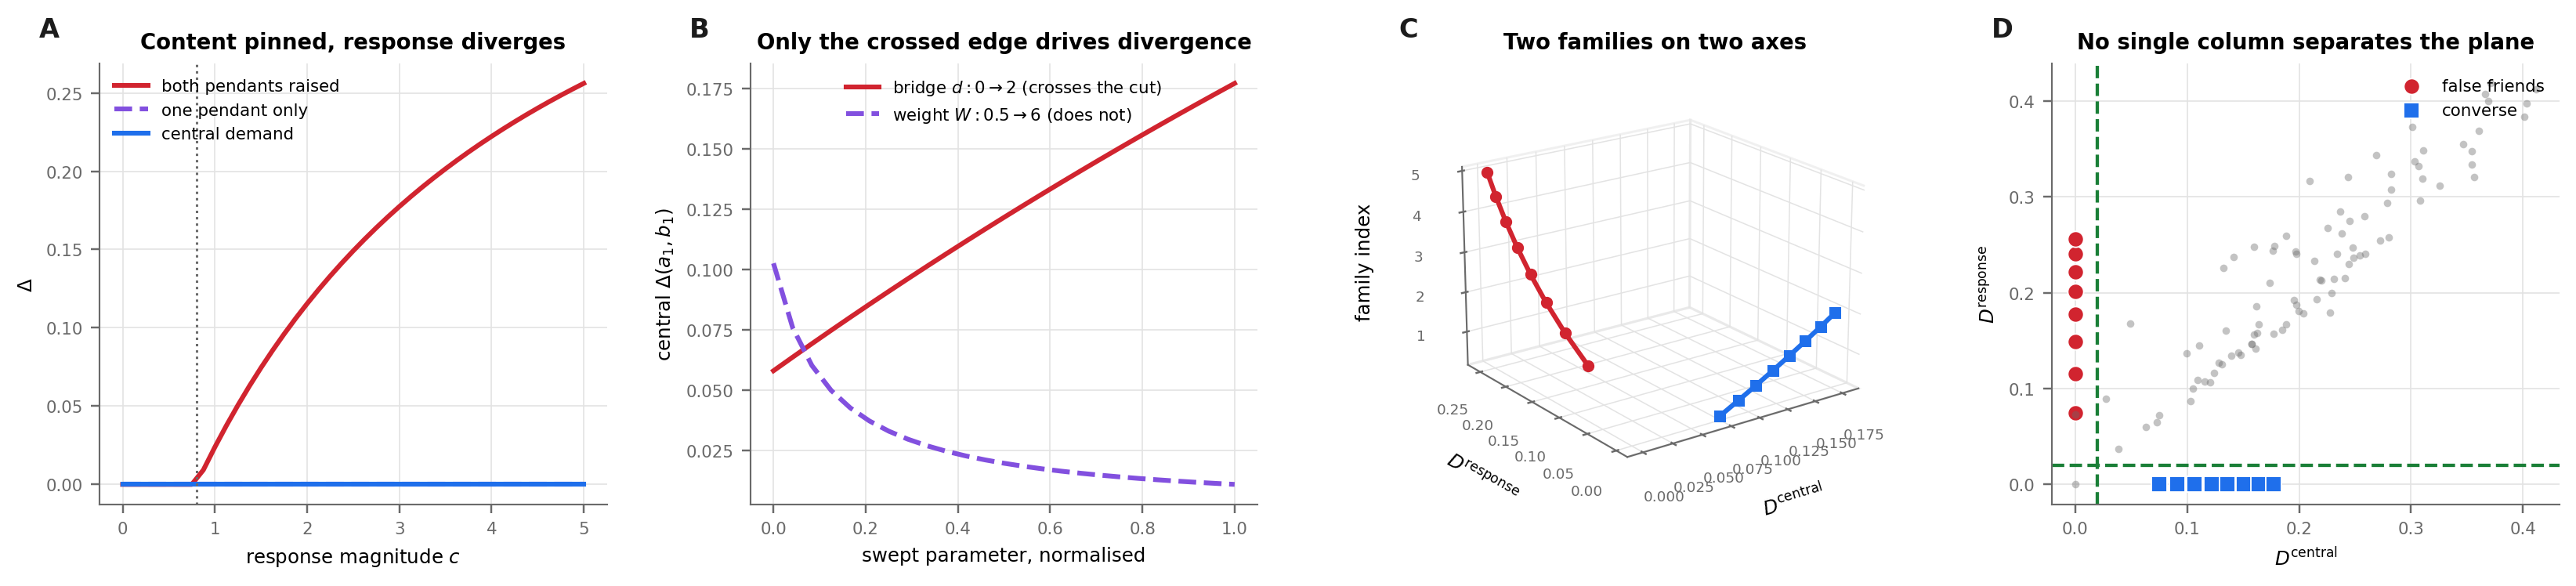
\includegraphics[width=\textwidth]{figures/panel_6_separation.png}
    \caption{\textbf{Content and response are orthogonal: each can be pinned at the floor while the other diverges without bound, so no single column can decide.}
    (\textbf{A})~The false-friend construction of \Cref{thm:falsefriend}. Raising \emph{both} pendant edges by $c$ drives the response demand from $0$ to $0.256$ while the central demand stays pinned at $0$ to machine precision for every $c$ --- content aligned exactly at the floor, response separating without bound (\Cref{rem:ffmeasured}, \eqref{eq:ffcurve}). The one-sided raise is plotted for contrast and never moves at all (maximum $0$ to machine precision): being pendant is essential, and raising a single edge leaves the cheapest cut free to route around it. That dashed vertical marks $w_f-\flo$, where the raised edges stop being the cheapest thing to sever.
    (\textbf{B})~The converse of \Cref{cor:converse}, both sweeps normalised to a common horizontal range so the two monotonicities can be read together. Perturbing the bridge --- the edge that crosses the minimising cut --- drives the central demand up from $0.058$ to $0.177$. Raising the intra-cluster weight $W$, which does not cross that cut, drives it \emph{down} from $0.103$ to $0.011$: the cut is constant while $\Om$ grows, so the normalised quantity falls. Only the crossed edge drives divergence. The direction of the second curve is the correction recorded in \Cref{sec:validation}, E17 --- our first attempt asserted the wrong monotonicity here and the sweep, not the argument, caught it.
    (\textbf{C})~The two families lifted onto the demand coordinates $(\dem^{\mathrm{central}},\dem^{\mathrm{response}})$ of \Cref{def:fourq}. The false-friend family lies along one axis with central demand $0$ to machine precision; the converse family lies along the other with response demand $0$ to machine precision. Each family is constant in one coordinate and unbounded in the other, so neither coordinate alone can separate its own family's members.
    (\textbf{D})~The consequence, drawn in the plane. Any criterion that is a function of $\dem^{\mathrm{central}}$ alone is constant on the first family; any function of $\dem^{\mathrm{response}}$ alone is constant on the second. The threshold lines at $\theta$ partition the plane into the quadrants of \Cref{def:fourq}, and the two families fall in different quadrants while agreeing on one coordinate each. This is \Cref{cor:orth} and \Cref{thm:four}: the four-column verdict separates what no single column can (\Cref{rem:orthmeasured}), and it is why \kw{align} takes a central pair and a response pair or does not typecheck.}
    \label{fig:panel6}
\end{figure*}

\begin{figure*}[!htbp]
    \centering
    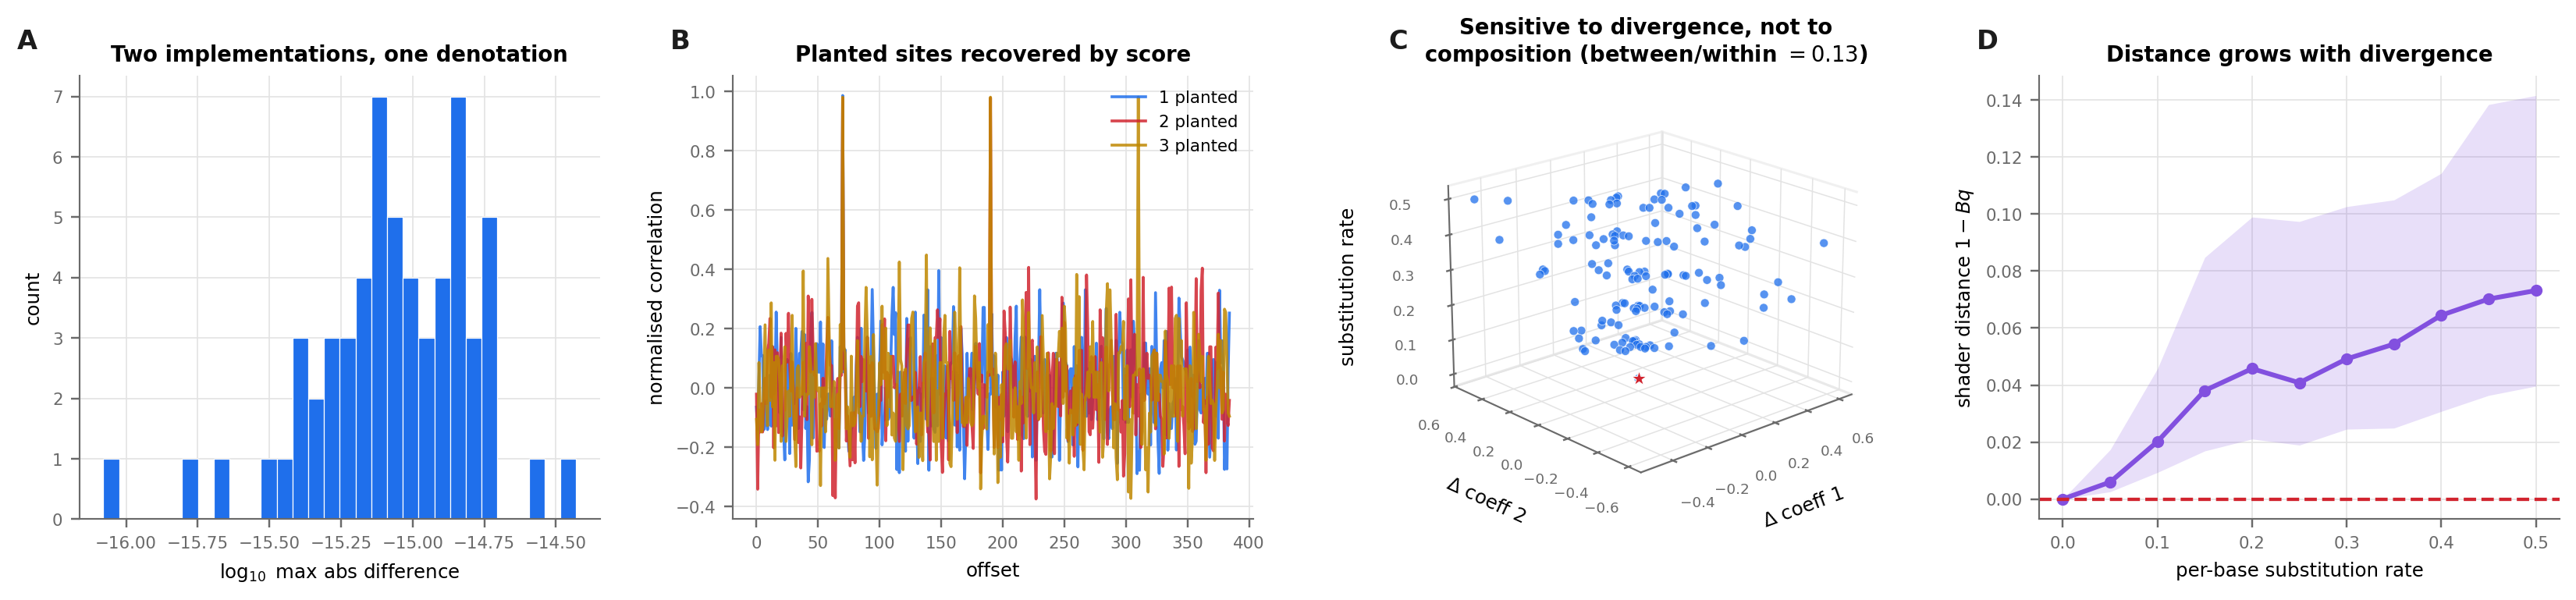
\includegraphics[width=\textwidth]{figures/panel_7_semantics.png}
    \caption{\textbf{The semantic operations are implementation-independent, recover planted structure, and are sensitive to divergence rather than to composition.}
    (\textbf{A})~Two independent implementations of cross-correlation --- direct summation and the FFT route --- over $60$ random query/target pairs, as the distribution of $\log_{10}$ maximum absolute difference. The largest disagreement anywhere is $3.7\times10^{-15}$, at the level of double-precision rounding. \Cref{def:xcorr} therefore names a denotation and not a routine: a synopsis program that specifies \texttt{xcorr} is specifying what is computed, and an implementation is free to choose how (\Cref{sec:semantics}).
    (\textbf{B})~Planted-motif recovery. A $16$-base motif is planted at one, two and three sites in a random background and located by normalised correlation; each planted site appears as a distinct peak at its offset, and the number of peaks tracks the number of plantings. This is what \kw{detect} \kw{peaks} consumes, and why its parameters --- $z$, minimum distance, minimum score --- are required in the program text rather than defaulted (\Cref{rule:nodefault}, \Cref{thm:params}).
    (\textbf{C})~What the spectral embedding of \Cref{def:spectral} is, and is not, sensitive to. Corrupted replicates are drawn as a cloud per substitution rate, plotted as displacement from their \emph{own} uncorrupted reference (star at the origin); the cloud spreads from the origin as the rate rises. Composition, by contrast, it does not separate: the mean distance between AT-rich, random and GC-rich family centres is only $0.127$ times the mean spread \emph{within} a family, so a family scatter would be three interleaved clouds. We plot the measured ratio in the axis rather than asserting a separation the embedding does not have --- reporting the null is the same discipline that governs \Cref{sec:open}.
    (\textbf{D})~Shader distance (\Cref{def:shader}) against per-base substitution rate, median with interquartile band over $300$ draws per rate spanning $30$ independent references. The median rises from $0$ at rate $0$ to $0.073$ at rate $0.5$, with $1$ inversion in $10$ steps. Sampling matters here: at $40$ draws off a single reference the curve is dominated by that reference's own accidents and is not monotone, which is why the reference set rather than the replicate count was enlarged. The sweep stops at $0.5$ because beyond it a sequence is closer to unrelated than to its reference and the statistic saturates.}
    \label{fig:panel7}
\end{figure*}

\begin{figure*}[!htbp]
    \centering
    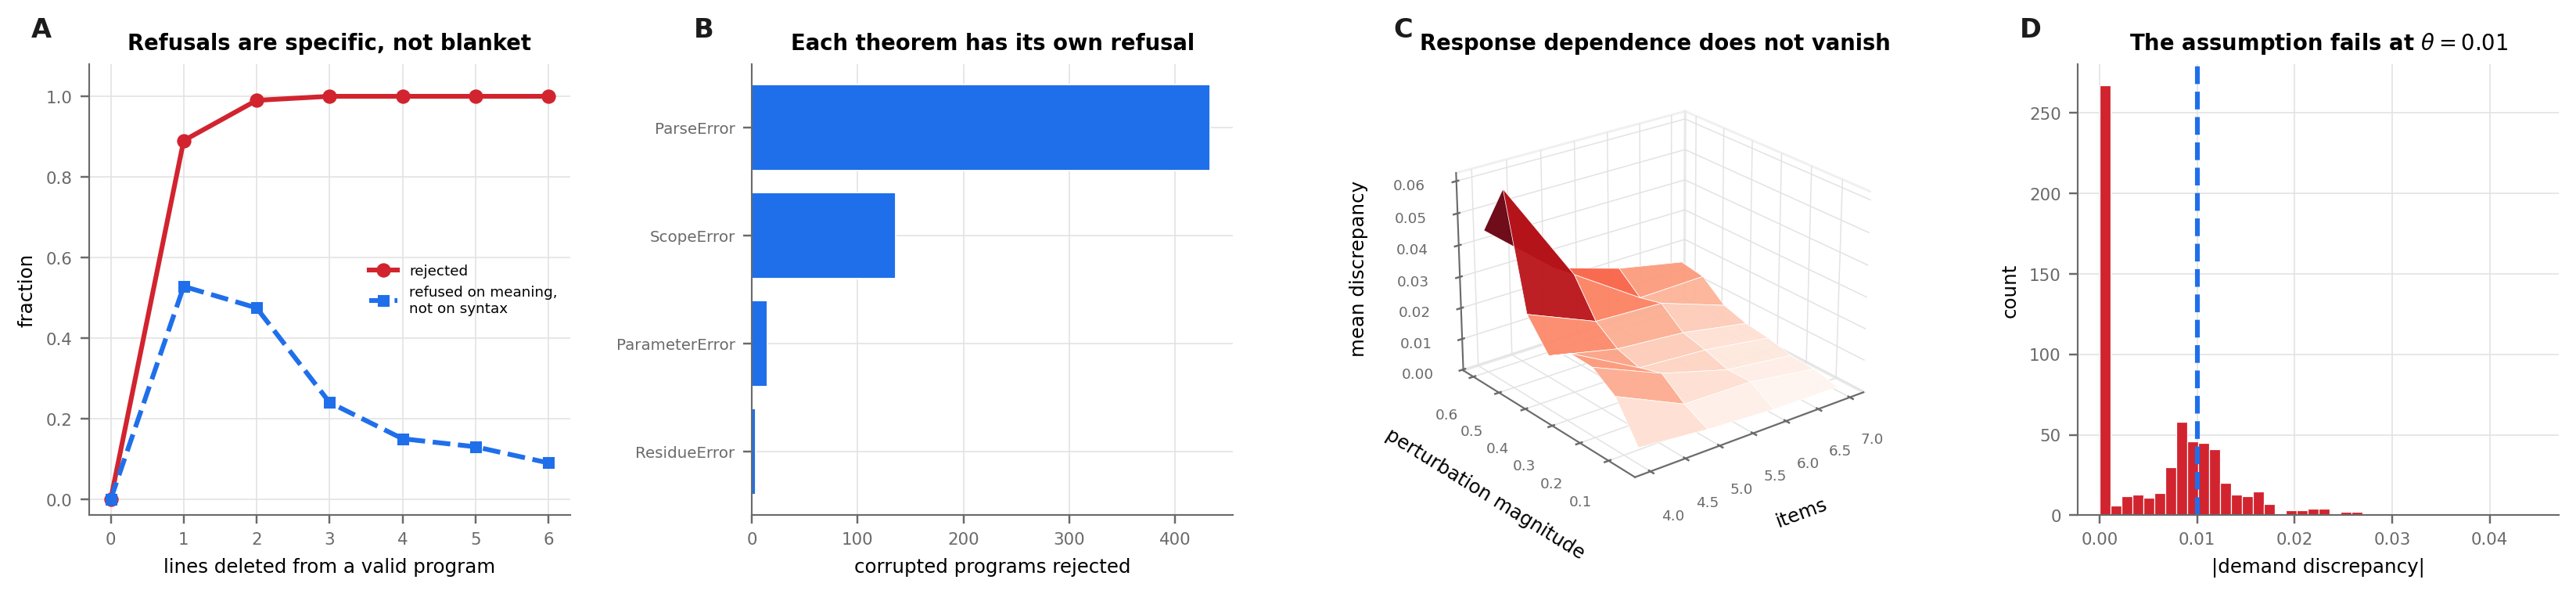
\includegraphics[width=\textwidth]{figures/panel_8_language_open.png}
    \caption{\textbf{The checker refuses wrong programs specifically rather than blanketly, and response independence --- the framework's principal open problem --- fails at the stated threshold.}
    (\textbf{A})~The checker's response to progressive corruption. Valid programs are corrupted by deleting $k$ non-blank lines and the rejection rate is swept over $k$: it rises from $0.00$ at $k=0$ --- the corpus is valid, and nothing in it is refused --- to $1.00$, while the share of refusals attributable to \emph{meaning} rather than to syntax falls from $0.53$ to $0.09$. Both movements are required. A checker that rejected everything would show the first curve and not the second; that refusals start semantic and become syntactic as more structure is destroyed is the evidence that the rules are discriminating, not merely strict. All $16$ negative programs are rejected, each in its expected error class.
    (\textbf{B})~The refusals resolved by class. Each theorem of \Cref{sec:lang} has its own refusal: scope violations (\Cref{thm:scope}), arity violations of \kw{align} (\Cref{thm:arity}, \Cref{rule:arity}), missing required parameters (\Cref{thm:params}, \Cref{rule:nodefault}), and discarded residue (\Cref{rule:residue}). A program is not rejected by a general-purpose plausibility check but by the specific rule it breaks, which is what makes the rejection message actionable and the property provable.
    (\textbf{C})~Response independence as a surface. The mean discrepancy between two admissible responses --- formed by raising one or the other incident edge of an item by the same magnitude --- is plotted over structure size and perturbation magnitude. It ranges over $9.2\times10^{-4}$ to $6.1\times10^{-2}$ and nowhere approaches zero; it grows with perturbation magnitude and does not shrink with size. The dependence is systematic across the parameter space rather than an artefact of small or particular structures.
    (\textbf{D})~The same discrepancies against the decision threshold. Over $632$ comparisons only $71.2\%$ fall within $\theta=0.01$ (dashed line); the mean is $0.0061$ and the maximum $0.0449$, exceeding $\theta$ by more than four-fold. \Cref{ass:respind} therefore does not hold at this threshold, and by \Cref{prop:respind} the four-column verdict depends on which admissible response was constructed. The independently-run validation suite agrees (\Cref{sec:validation}, E32: $361$ comparisons, $77.8\%$ within $\theta$, maximum $0.036$). We report this as the framework's principal open problem (\Cref{sec:open}) rather than as a tuning failure: what is missing is a rule fixing the map from a unit to the perturbation it induces, not a better threshold or more data. Raising $\theta$ until the assumption passes would make the verdict depend on the threshold instead --- which is the same defect wearing a different name.}
    \label{fig:panel8}
\end{figure*}
